\section{Durchführung}
\subsection{Gedämpfte Schwingung}
In den Kreis \ref{fig:d1} wird ein einzelner Spannungspuls in Form
von Rechteckwechselspannung simuliert, sodass die
abnehmenden Amplituden der Spannungskurve nach der Zeit von dem Osziloskop abgelesen werden können.
\label{sec:Durchführung}
\begin{figure}[H]
  \centering
  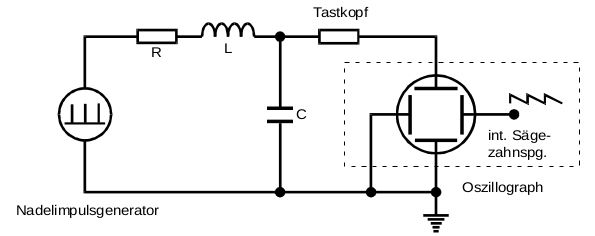
\includegraphics{content/images/d1.png}
  \caption{Schaltkreis gedämpfte Schwingung experimentell\cite{anleitung}.}
  \label{fig:d1}
\end{figure}

\subsection{aperiodischer Grenzfall}
Bei Einspeisen einer Rechteckwechselspannung in \ref{fig:d2} wird der verstellbare
Widerstand so eingestellt, dass kein Überschwingen der Einhüllenden mehr
vom Osziloskop abzulesen ist.
\begin{figure}[H]
  \centering
  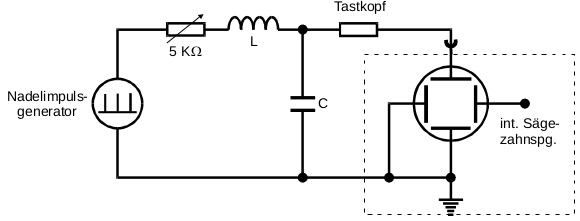
\includegraphics{content/images/d2.png}
  \caption{Schaltkreis Bestimmung des aperiodischen Grenzfalls experimentell\cite{anleitung}.}
  \label{fig:d2}
\end{figure}

\subsection{Frequenzabhängige Kondensatorspannung}
\label{sec:d3}
Die Kondensatorspannung in \ref{fig:d3} wird für verschiedene Frequenzen abgelesen bis sich nach
Bildung eines Maximums an der Eigenfrequenz des Schwingkreises die Kondensatorspannung wieder dem
anfänglichen Wert nähert, sodass eine Glockenkurve erkennbar ist.
\begin{figure}[H]
  \centering
  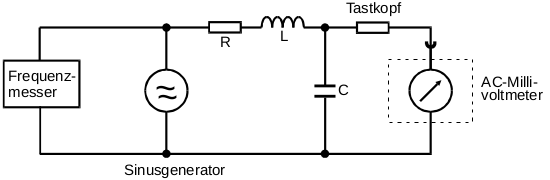
\includegraphics{content/images/d3.png}
  \caption{Schaltkreis Kondensatorspannung zu Frequenz experimentell\cite{anleitung}.}
  \label{fig:d3}
\end{figure}

\subsection{Frequenzabhängige Phase}
Erreger- und Kondensatorspannung in \ref{fig:d4} werden auf dem Oszilloskop übereinander gelegt
und die Phasendifferenz wird für dieselben Frequenzen $\nu$ wie in \ref{sec:d3} notiert.
\begin{figure}[H]
  \centering
  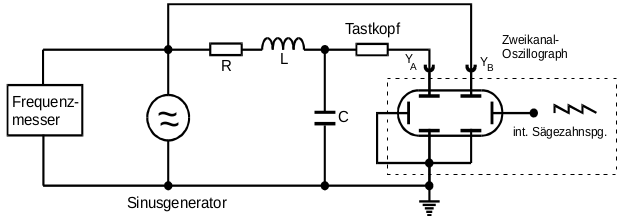
\includegraphics{content/images/d4.png}
  \caption{Schaltkreis Phase zwischen Erreger- und Kondensatorspannung zu Frequenz experimentell\cite{anleitung}.}
  \label{fig:d4}
\end{figure}
